
Power modeling has received a lot of attention from researchers and developers as it
provides a quick and robust way to understand the power behavior of a system.  A common
approach for predicting power consumption consists in the usage of Performance Monitoring
Counters
(PMC)~\cite{Bertran:2010:DRP:1810085.1810108,Singh:2009:RTP:1577129.1577137,Bellosa:2000:BED:566726.566736,Bircher:2012:CSP:2196827.2196987,Bircher:2005:RIM:1077603.1077668,Li:2003:RME:781027.781048},
since sampling PMC does not introduce significant power
interference~\cite{Joseph:2001:RPE:383082.383119,Isci:2003:RPM:956417.956567} and
PMC-based prediction models decompose a chip into several components in terms of power
consumption~\cite{Bertran:2010:DRP:1810085.1810108}.  While power prediction models are
employed to find the best tradeoff between power and
performance~\cite{Gholkar:2016:PTH:2967938.2967961}, we are not aware of any previous work
that uses variability-aware power models to guide job scheduling decisions.  

%In the rest of the document, we consider a cluster to consist of multiple nodes, each with
%multiple sockets. Thus, the terms socket and CPU are used interchangeably.


\subsection{Power Ratio Model}
\label{sec:naive_model}

\begin{figure*}[!ht]
	\centering
\begin{subfigure}[b]{.45\textwidth}
  	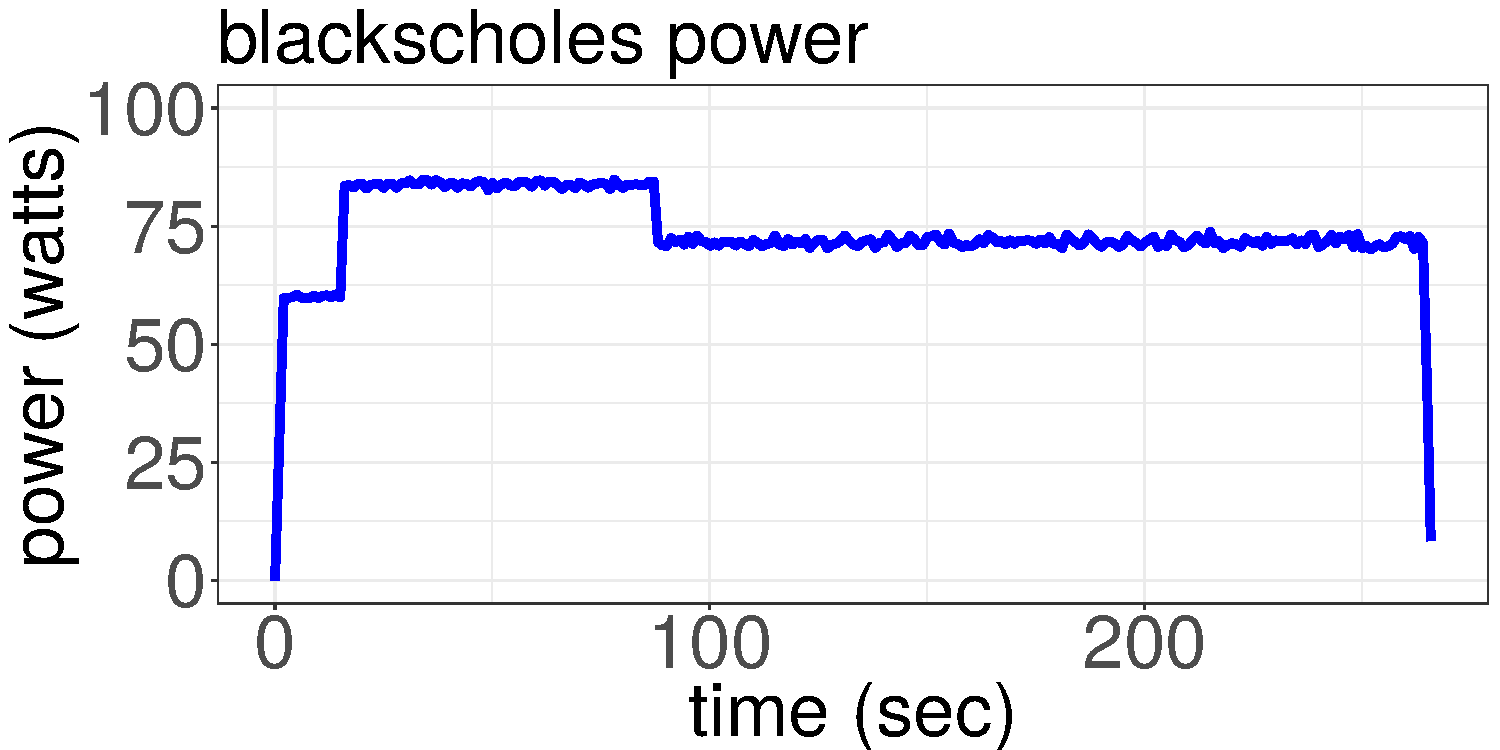
\includegraphics[width=\textwidth]{power_aware_job_scheduling/figures/activity_ratios/blackscholes_pkg_power}
  \end{subfigure}%
~
	\begin{subfigure}[b]{.45\textwidth}
  	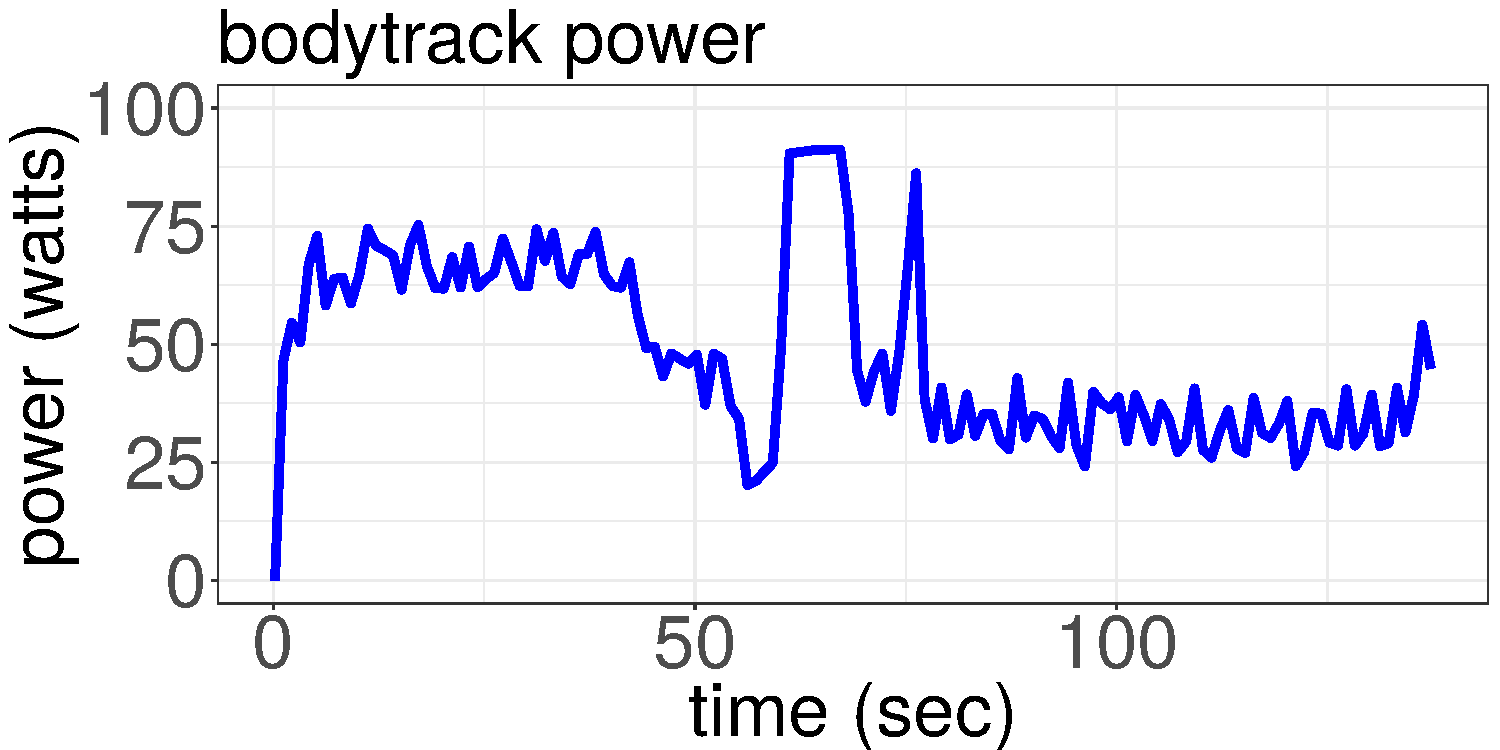
\includegraphics[width=\textwidth]{power_aware_job_scheduling/figures/activity_ratios/bodytrack_pkg_power}
	\end{subfigure}%
\vspace{0.1cm}
	\begin{subfigure}[b]{.45\textwidth}
  	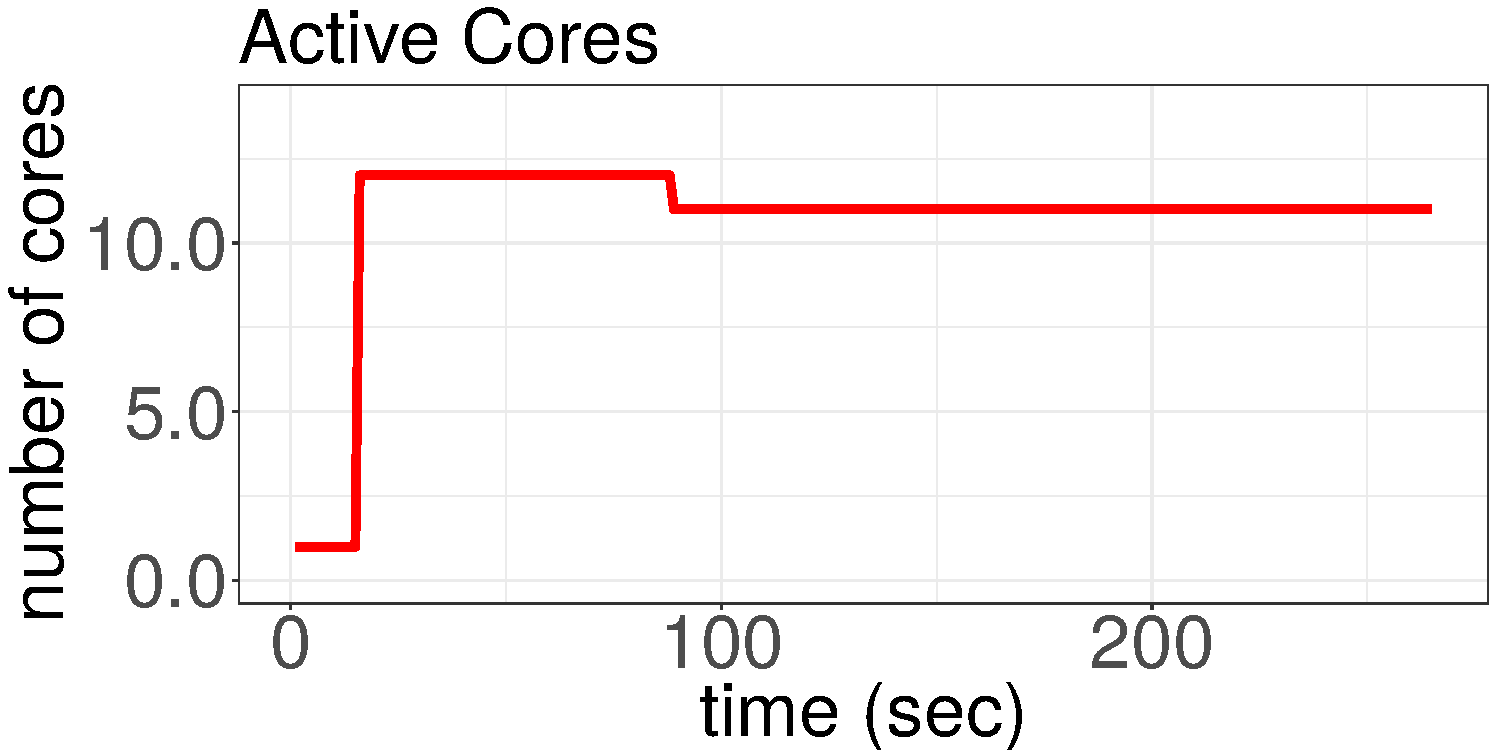
\includegraphics[width=\textwidth]{power_aware_job_scheduling/figures/activity_ratios/blackscholes_CORES}
  \end{subfigure}%
~
	\begin{subfigure}[b]{.45\textwidth}
  	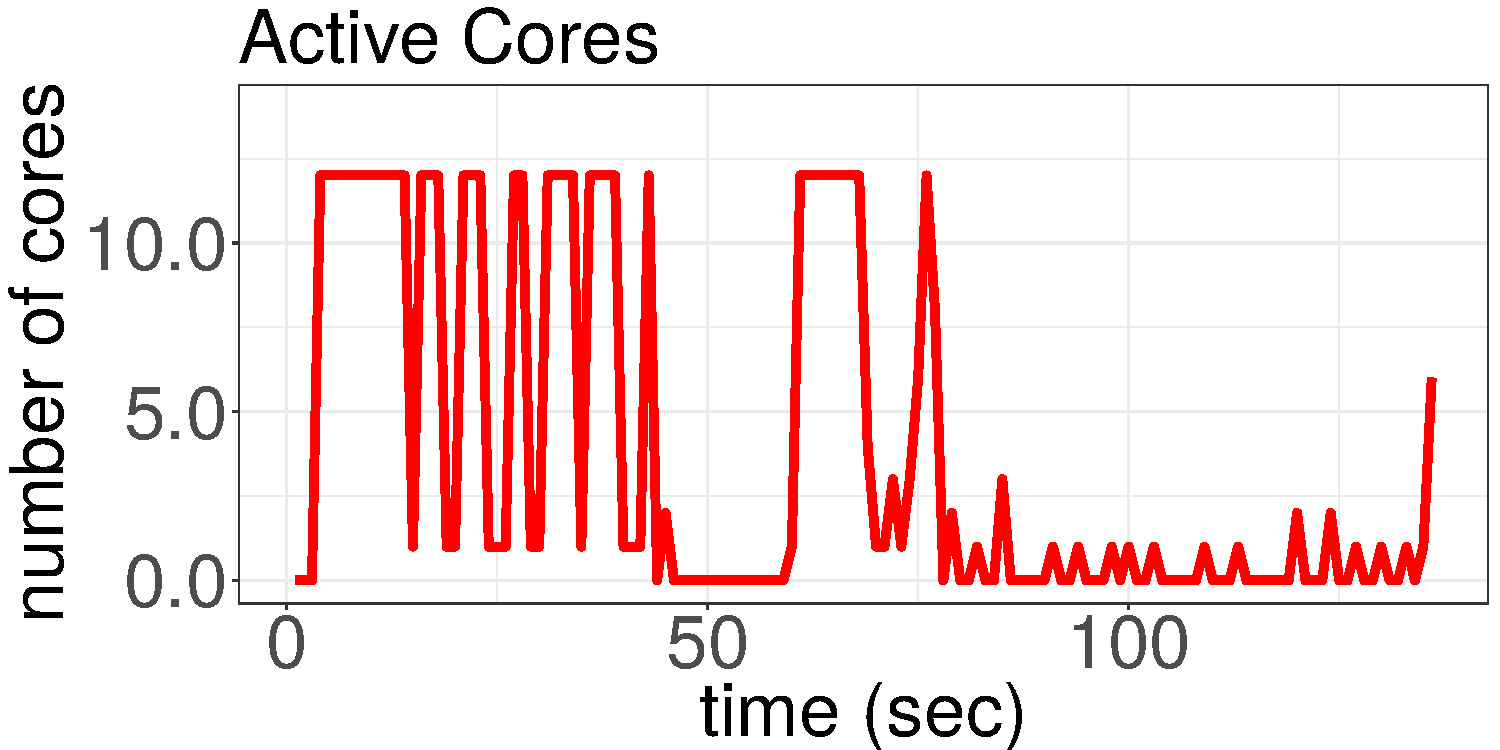
\includegraphics[width=\textwidth]{power_aware_job_scheduling/figures/activity_ratios/bodytrack_CORES}
  \end{subfigure}%
\vspace{0.1cm}
	\begin{subfigure}[b]{.45\textwidth}
  	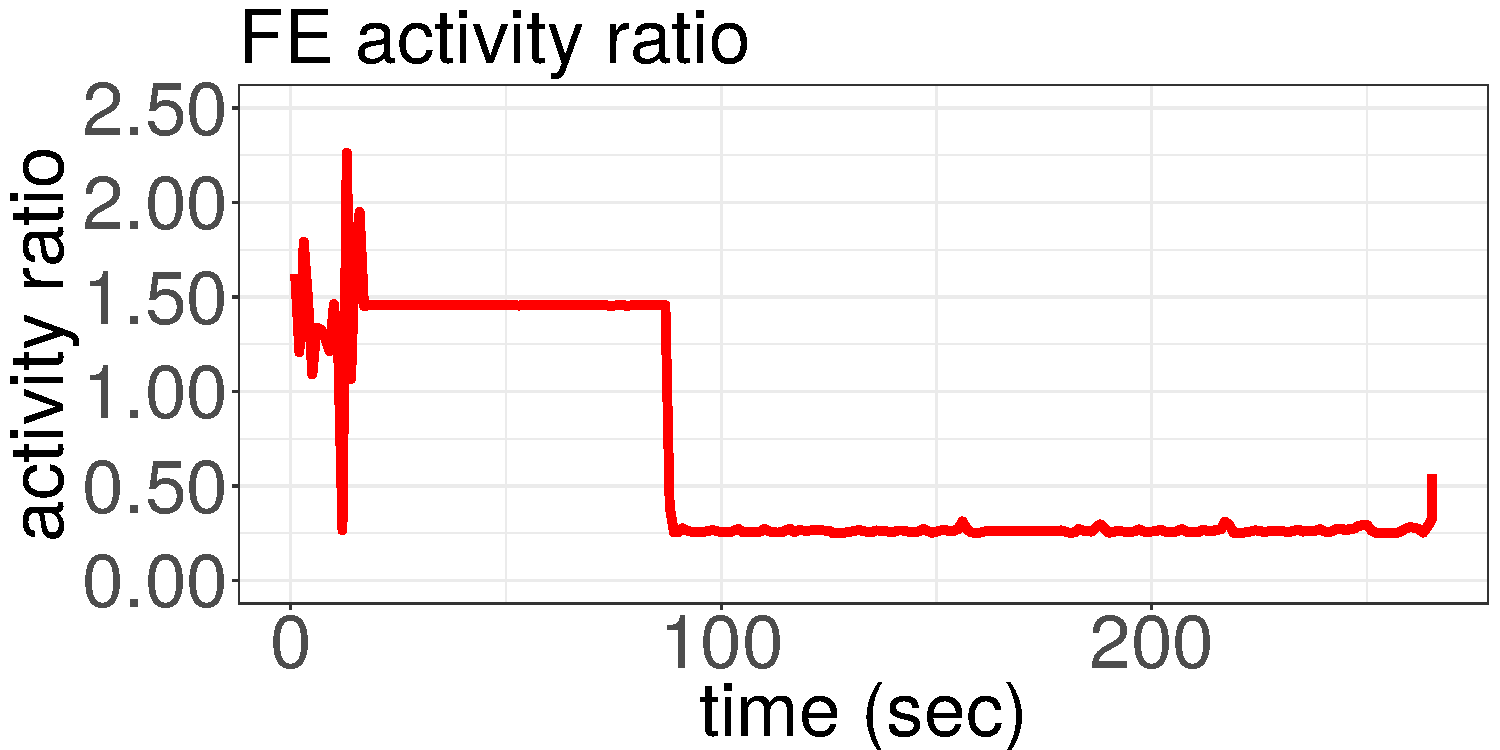
\includegraphics[width=\textwidth]{power_aware_job_scheduling/figures/activity_ratios/blackscholes_IPC}
  \end{subfigure}%
~
	\begin{subfigure}[b]{.45\textwidth}
  	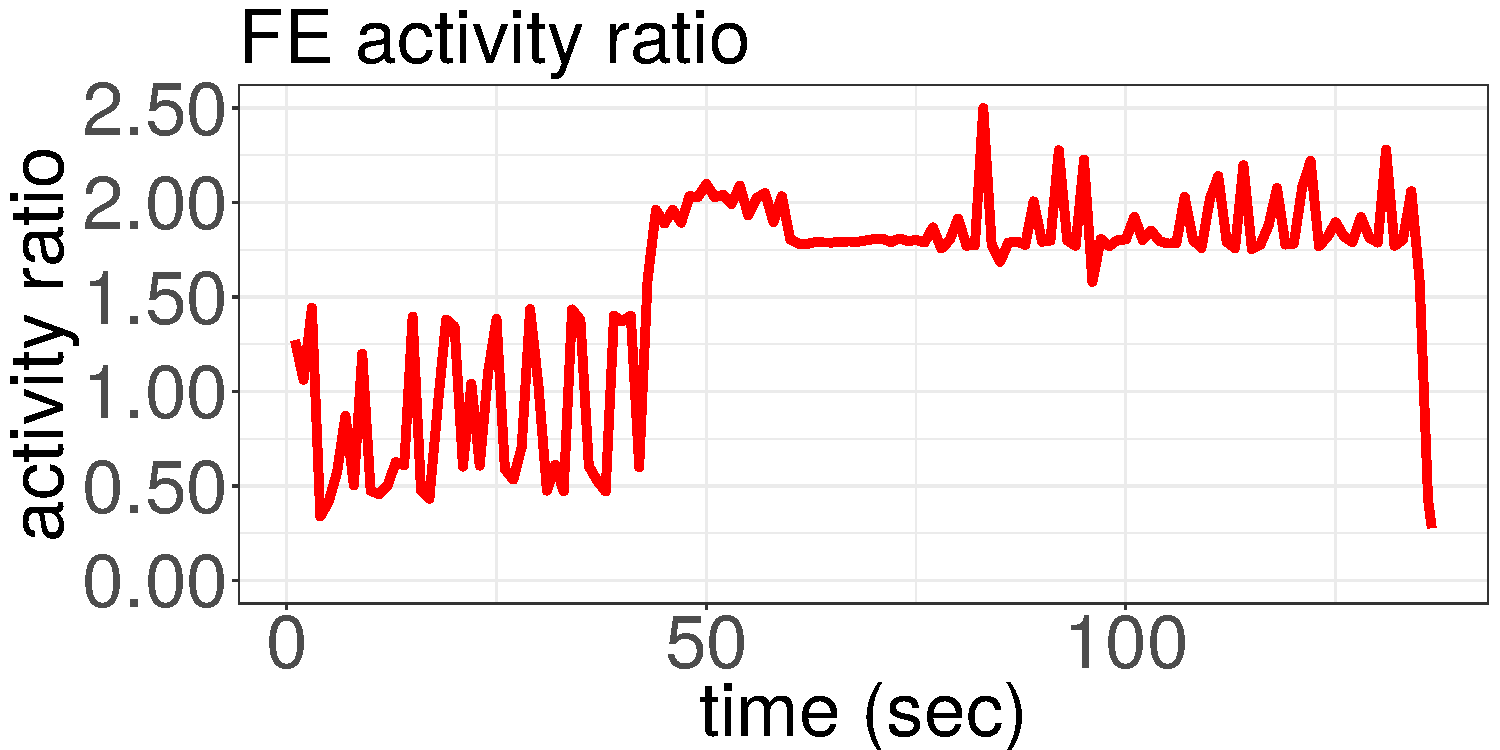
\includegraphics[width=\textwidth]{power_aware_job_scheduling/figures/activity_ratios/bodytrack_IPC}
  \end{subfigure}%
\vspace{0.1cm}
%	\begin{subfigure}[b]{.45\textwidth}
%  	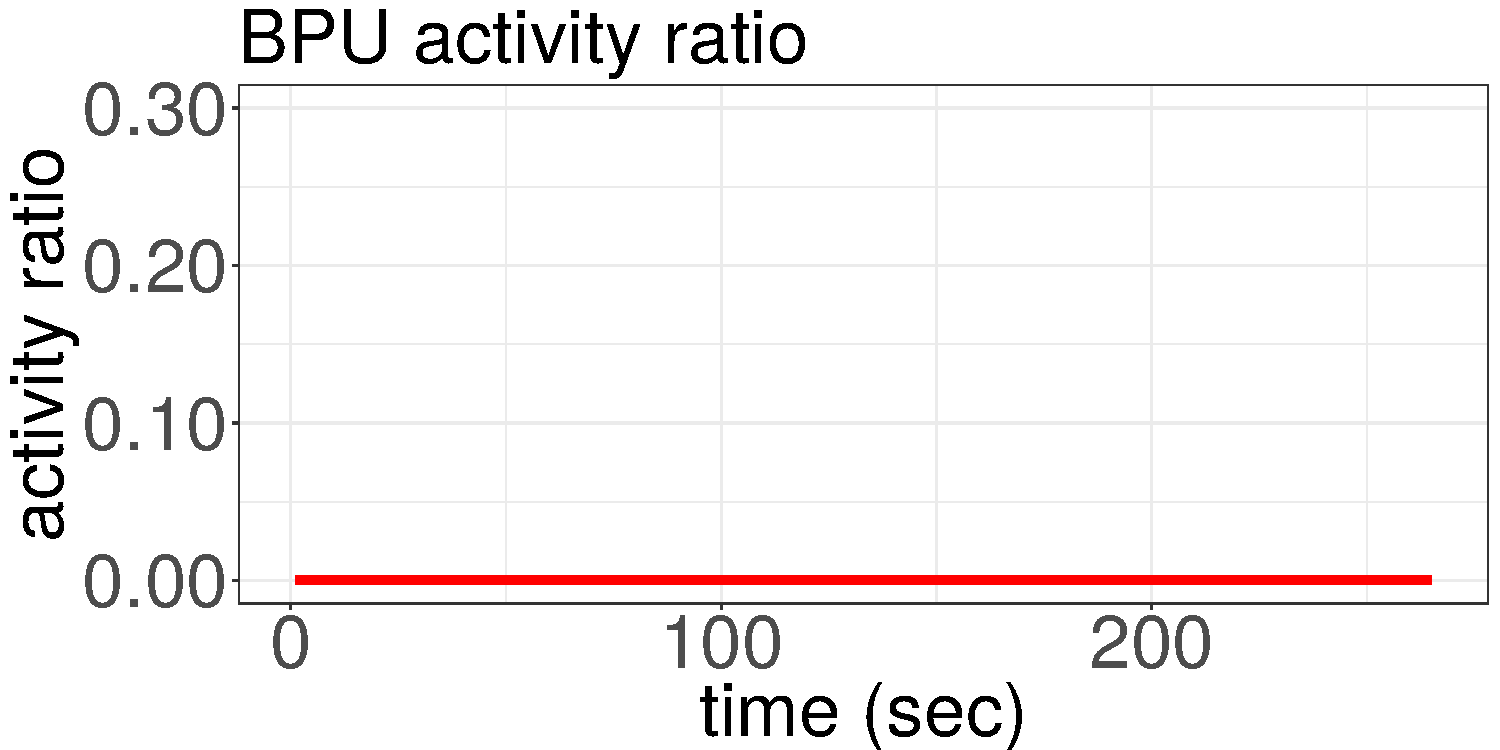
\includegraphics[width=\textwidth]{power_aware_job_scheduling/figures/activity_ratios/blackscholes_BPU}
%  \end{subfigure}%
%~
%	\begin{subfigure}[b]{.45\textwidth}
%  	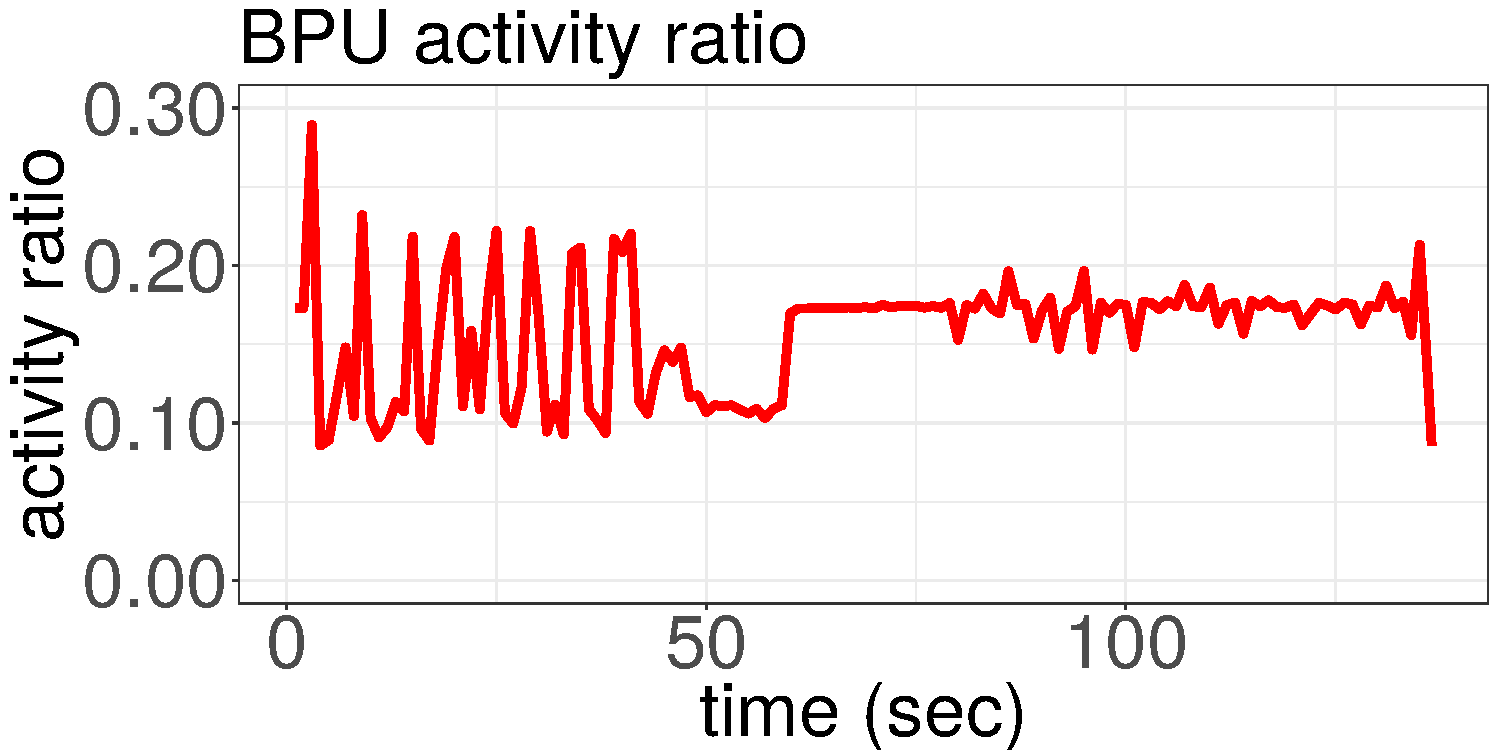
\includegraphics[width=\textwidth]{power_aware_job_scheduling/figures/activity_ratios/bodytrack_BPU}
%  \end{subfigure}%
%~
%	\begin{subfigure}[b]{.45\textwidth}
%	  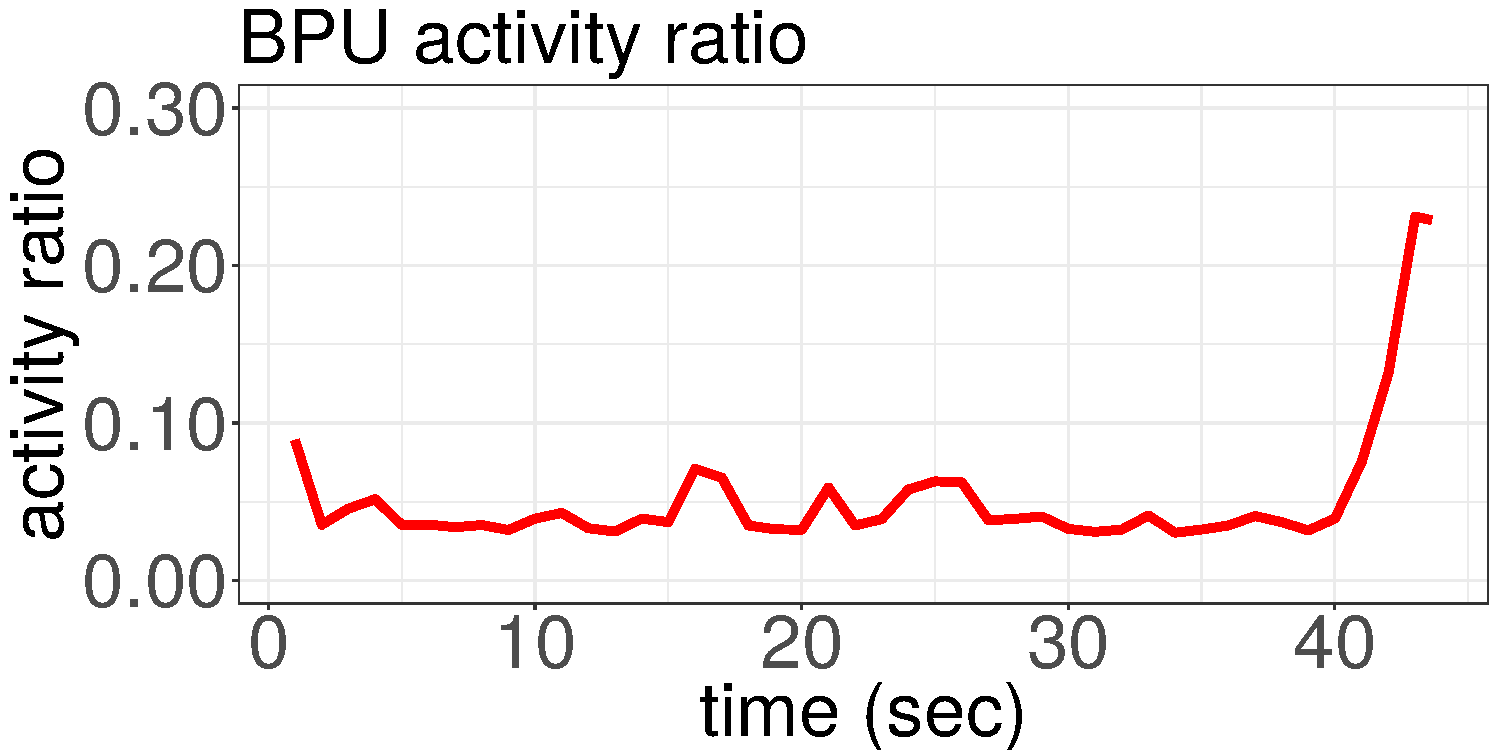
\includegraphics[width=\textwidth]{{power_aware_job_scheduling/figures/activity_ratios/lu-mz_C.16_BPU}.pdf}
%	\end{subfigure}%
%~
%	\begin{subfigure}[b]{.45\textwidth}
%	  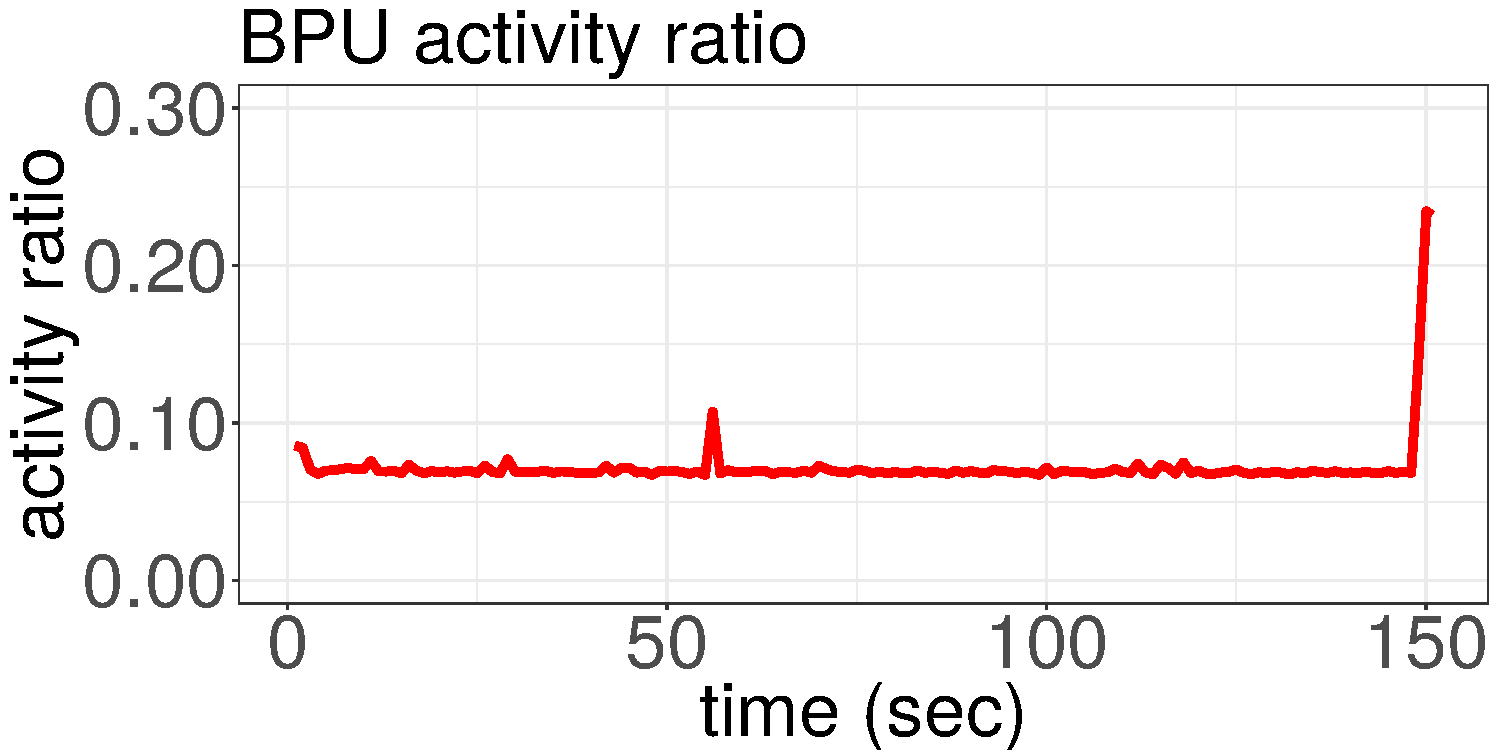
\includegraphics[width=\textwidth]{{power_aware_job_scheduling/figures/activity_ratios/sp-mz_D.8_BPU}.pdf}
%	\end{subfigure}%
%\vspace{0.1cm}
	\begin{subfigure}[b]{.45\textwidth}
  	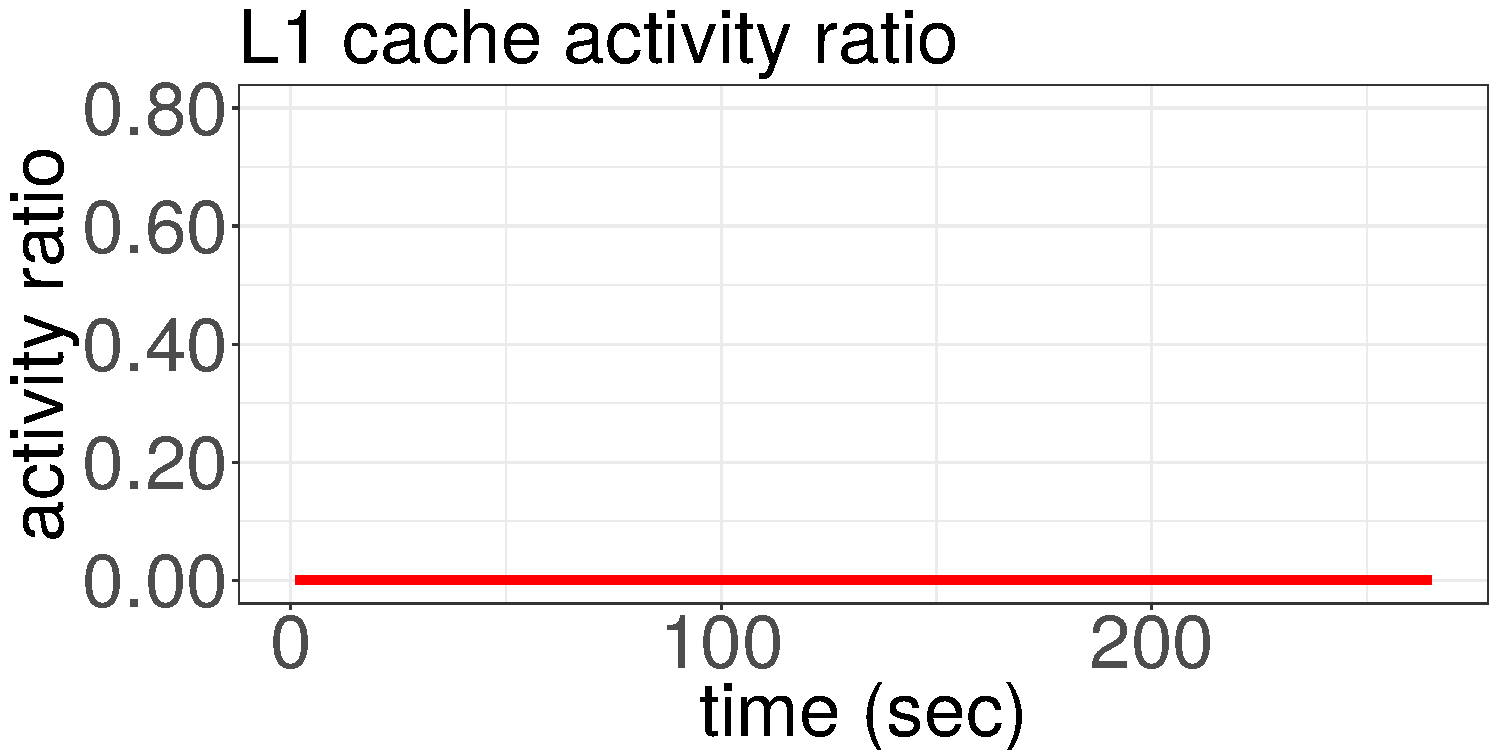
\includegraphics[width=\textwidth]{power_aware_job_scheduling/figures/activity_ratios/blackscholes_L1}
  \end{subfigure}%
~
	\begin{subfigure}[b]{.45\textwidth}
  	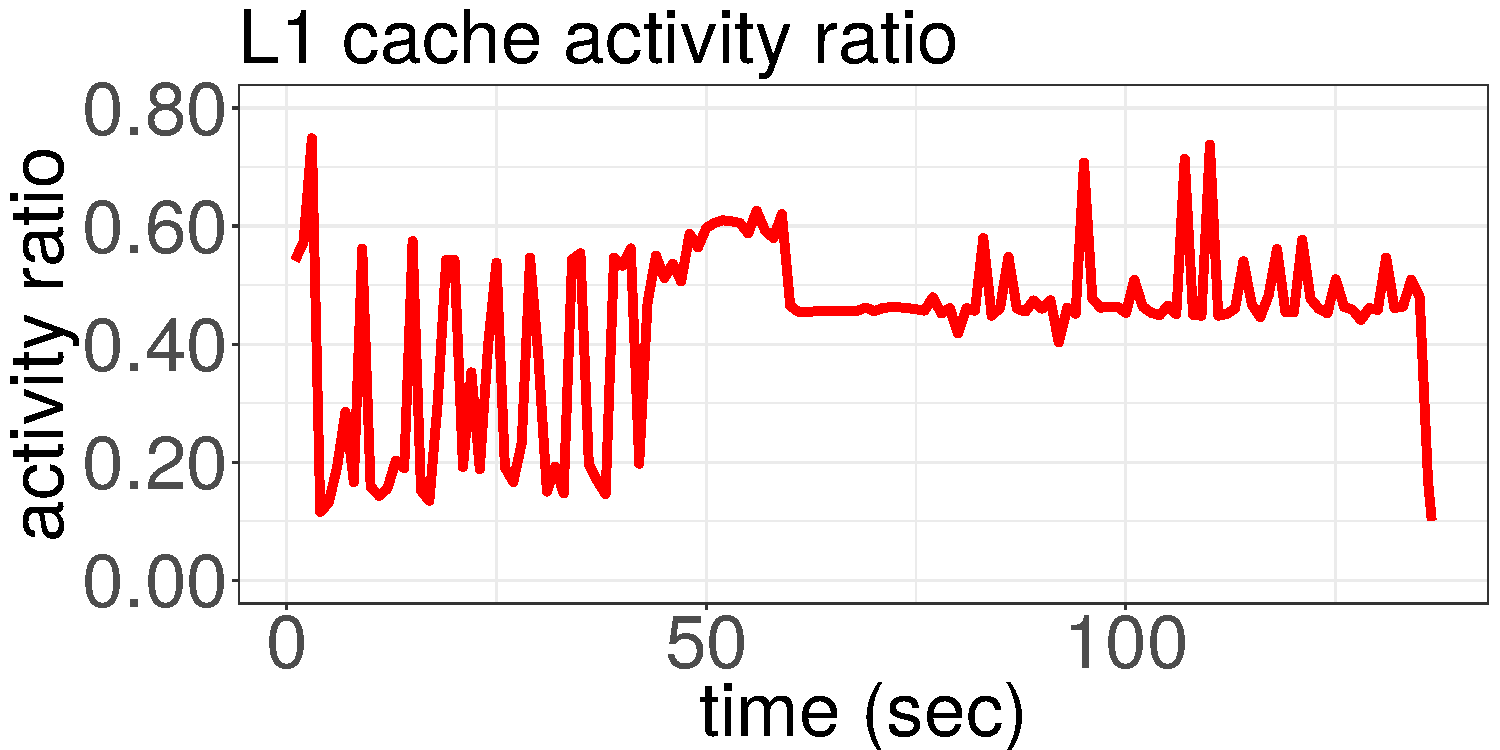
\includegraphics[width=\textwidth]{power_aware_job_scheduling/figures/activity_ratios/bodytrack_MEM}
  \end{subfigure}%

	\caption{Power, active cores and component activity ratio traces when running on 12
cores of a single socket.  Architectural components shown are the fetch unit (FE) and L1
cache.  The activity ratios are the number of retired micro operations per unhalted cycle,
relevant to each architectural component.  In the case of cores, activity ratio is the
number of active cores.  For memory the activity ratio is measured as the number of
references (for caches) or LLC misses (for main memory) per cycle.}
	\label{fig:component_activity_ratios_1}
	%\vspace{-.3cm}
\end{figure*}


\begin{figure*}[!ht]
	\centering
	\begin{subfigure}[b]{.45\textwidth}
	  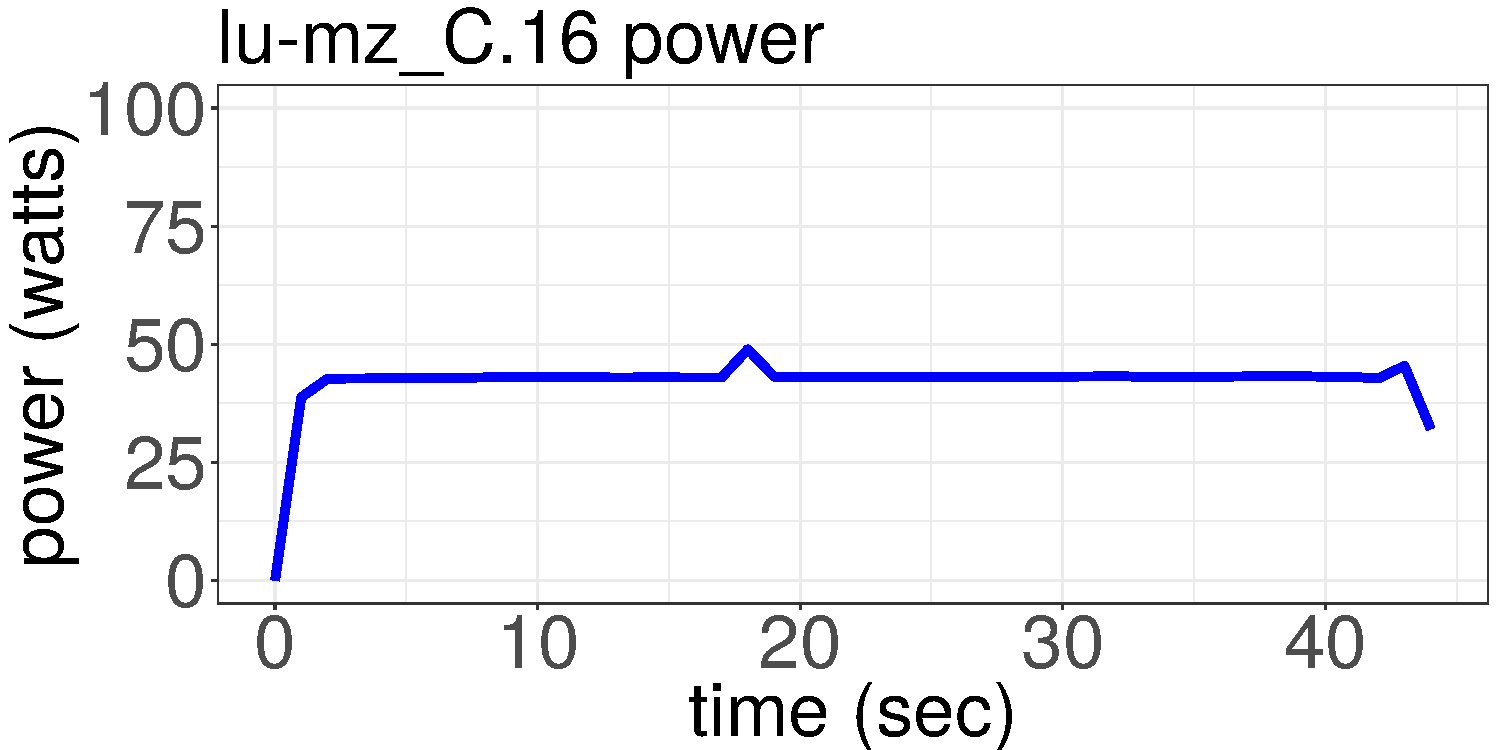
\includegraphics[width=\textwidth]{{power_aware_job_scheduling/figures/activity_ratios/lu-mz_C.16_pkg_power}.pdf}
	\end{subfigure}%
~
	\begin{subfigure}[b]{.45\textwidth}
	  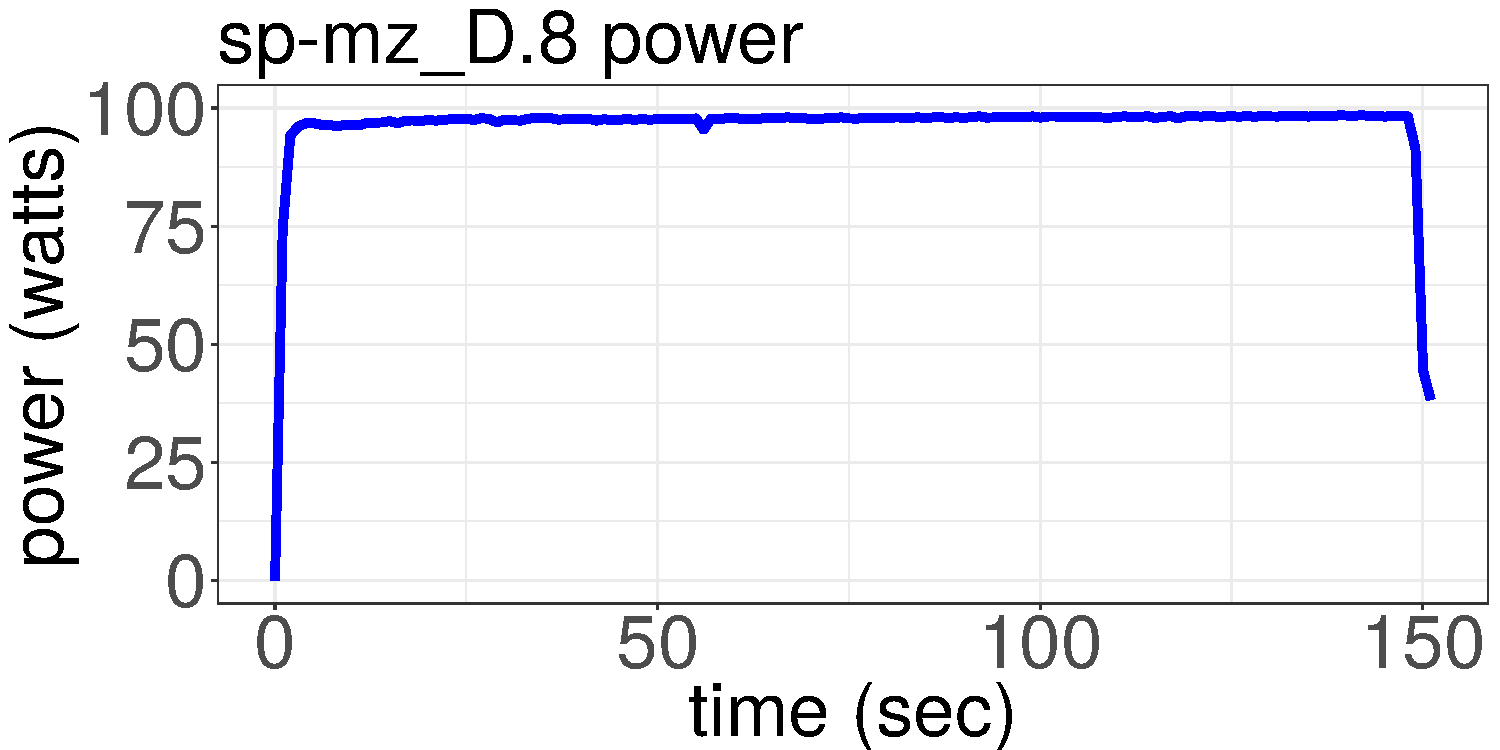
\includegraphics[width=\textwidth]{{power_aware_job_scheduling/figures/activity_ratios/sp-mz_D.8_pkg_power}.pdf}
	\end{subfigure}%
\vspace{0.1cm}
	\begin{subfigure}[b]{.45\textwidth}
	  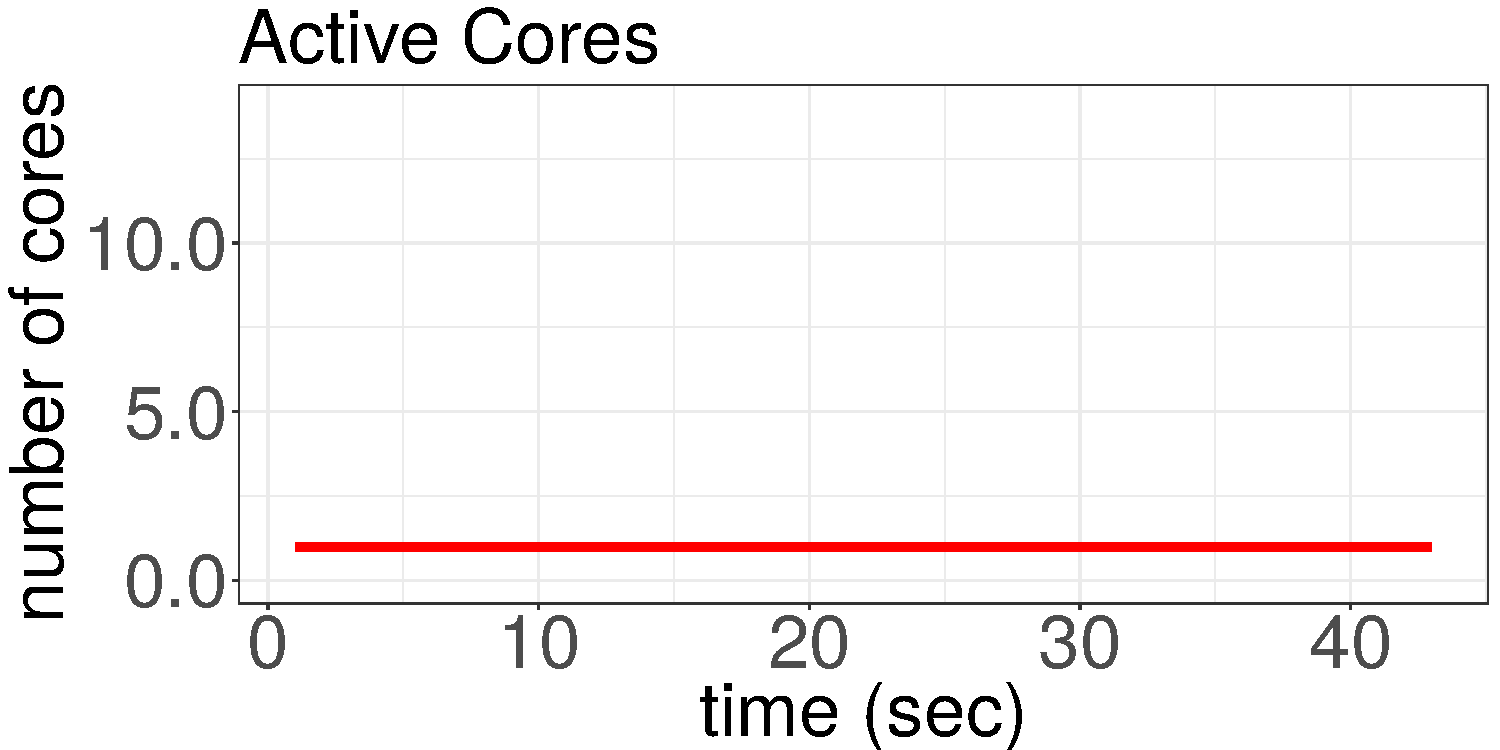
\includegraphics[width=\textwidth]{{power_aware_job_scheduling/figures/activity_ratios/lu-mz_C.16_CORES}.pdf}
	\end{subfigure}%
~
	\begin{subfigure}[b]{.45\textwidth}
	  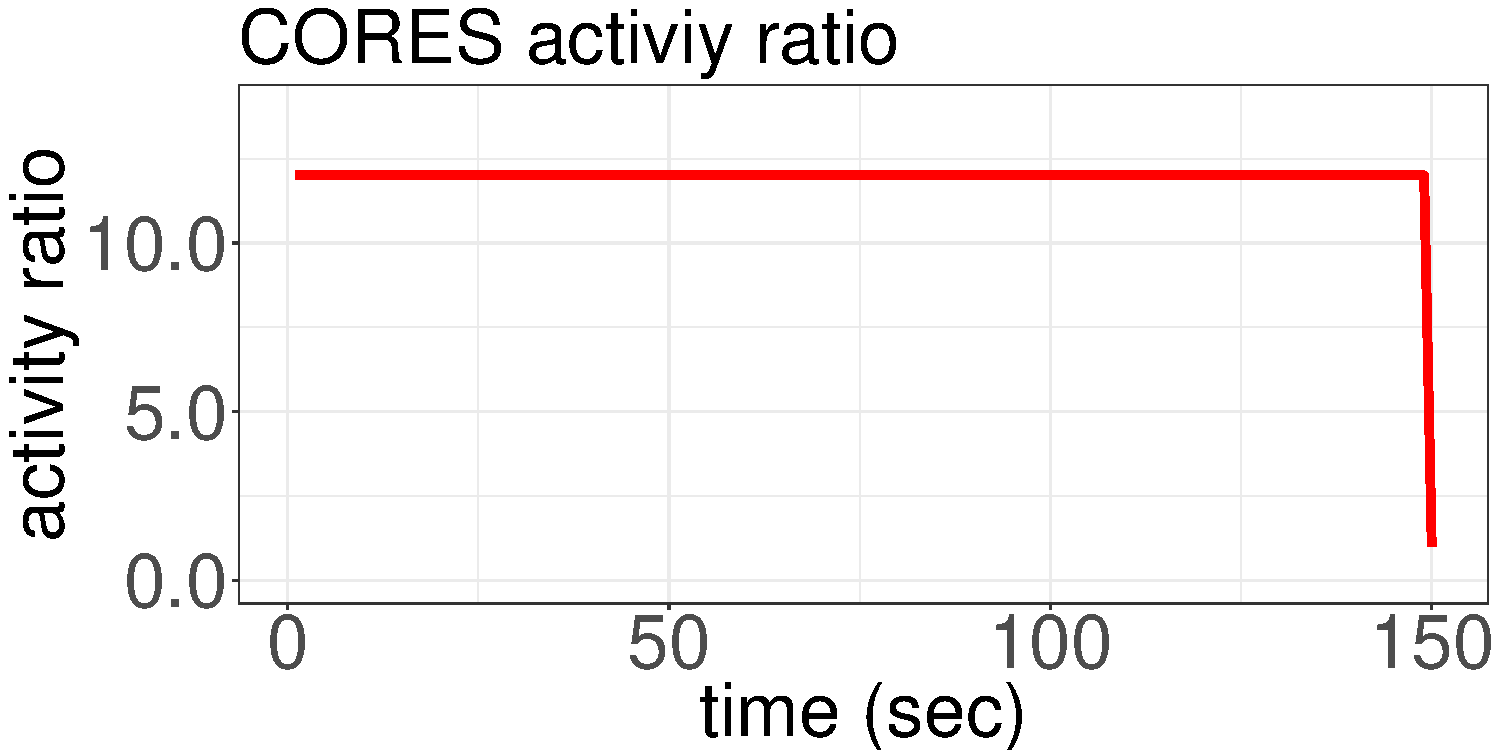
\includegraphics[width=\textwidth]{{power_aware_job_scheduling/figures/activity_ratios/sp-mz_D.8_CORES}.pdf}
	\end{subfigure}%
\vspace{0.1cm}
	\begin{subfigure}[b]{.45\textwidth}
	  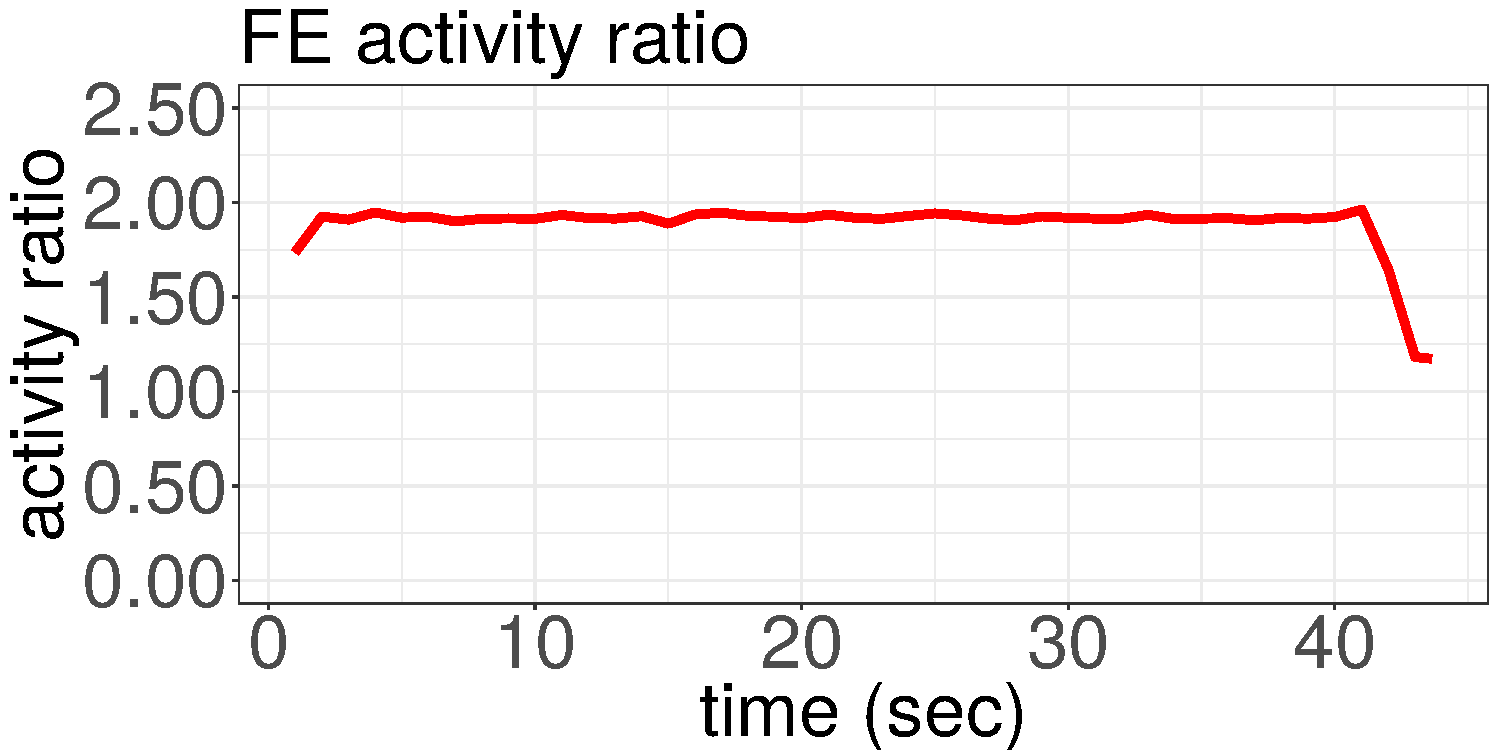
\includegraphics[width=\textwidth]{{power_aware_job_scheduling/figures/activity_ratios/lu-mz_C.16_IPC}.pdf}
	\end{subfigure}%
~
	\begin{subfigure}[b]{.45\textwidth}
	  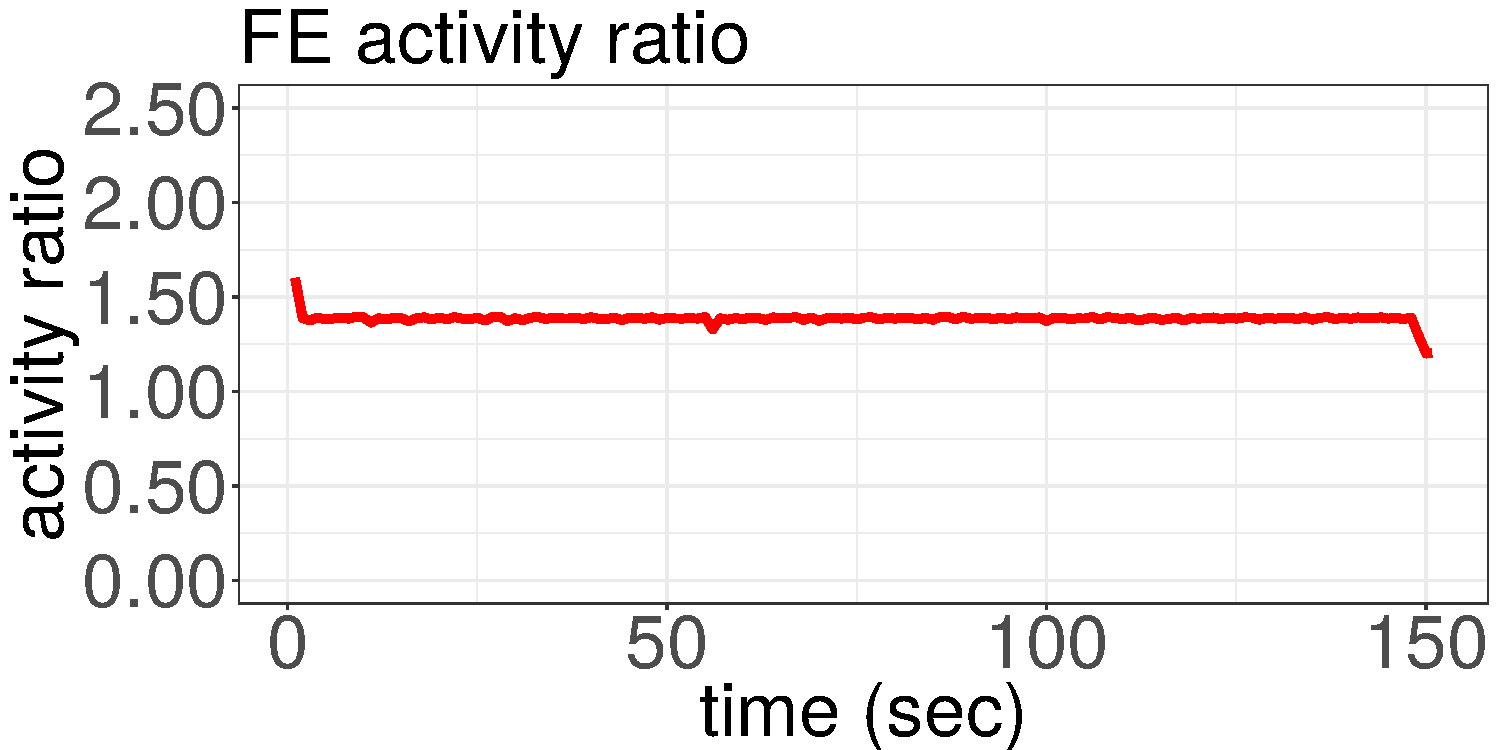
\includegraphics[width=\textwidth]{{power_aware_job_scheduling/figures/activity_ratios/sp-mz_D.8_IPC}.pdf}
	\end{subfigure}%
\vspace{0.1cm}
	\begin{subfigure}[b]{.45\textwidth}
	  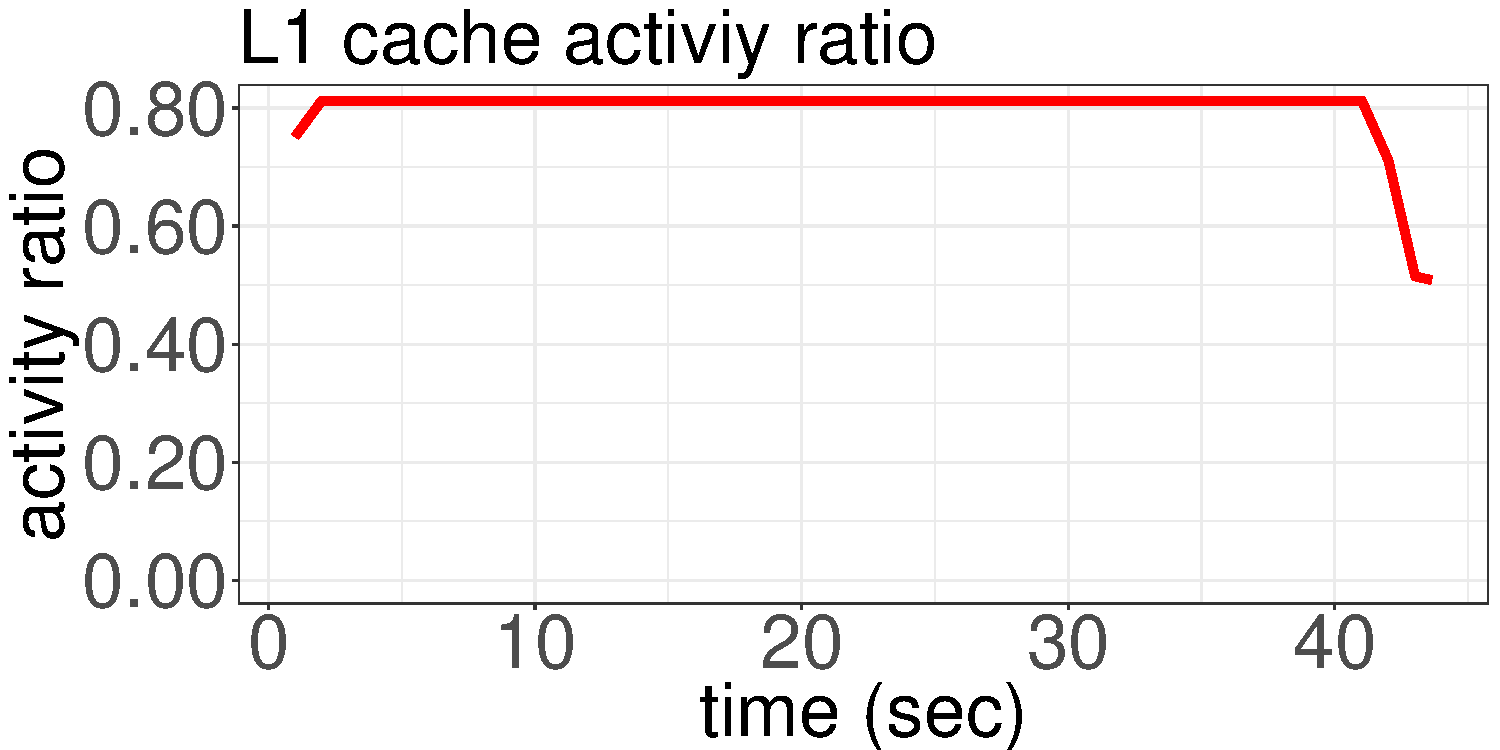
\includegraphics[width=\textwidth]{{power_aware_job_scheduling/figures/activity_ratios/lu-mz_C.16_MEM}.pdf}
	\end{subfigure}%
~
	\begin{subfigure}[b]{.45\textwidth}
	  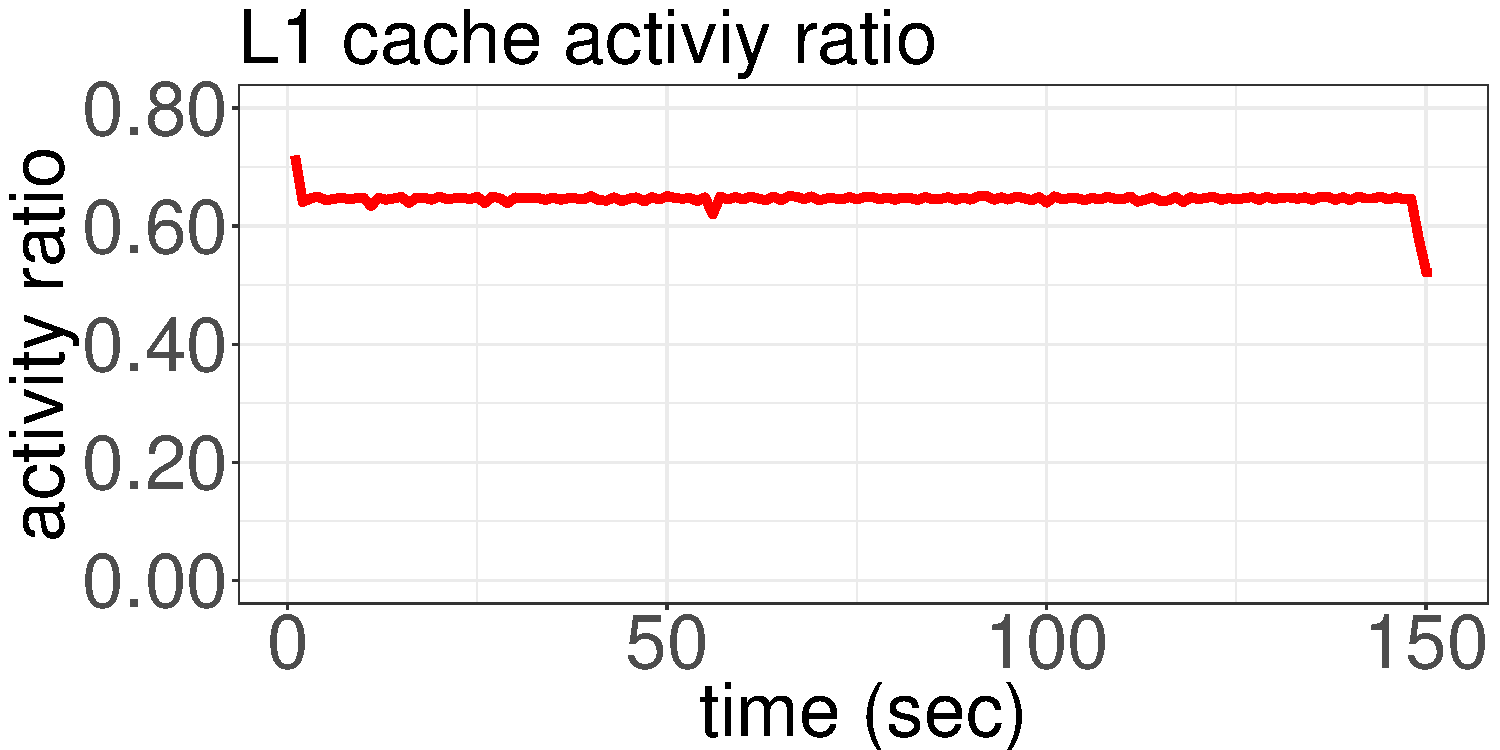
\includegraphics[width=\textwidth]{{power_aware_job_scheduling/figures/activity_ratios/sp-mz_D.8_MEM}.pdf}
	\end{subfigure}%

	\caption{Power, active cores and component activity ratio traces of MPI, multinode applications when running on 12 cores per socket.  Results show only activity on one socket, but the other sockets demonstrate similar behavior.
Architectural components shown are the fetch unit (FE) and L1
cache.  The activity ratios are the number of retired micro operations per unhalted cycle,
relevant to each architectural component.  In the case of cores, activity ratio is the
number of active cores.  For memory the activity ratio is measured as the number of
references (for caches) or LLC misses (for main memory) per cycle.  For multi-node
applications  PMC data is collected for all the processes and individual predictions 
are made for each socket.}
	\label{fig:component_activity_ratios_2}
	%\vspace{-.3cm}
\end{figure*}



\par
Our first (baseline) model attempts to circumvent the relative complexity of dealing with
manufacturing variability by assuming that all applications are impacted the same by it.
It uses a PMC-based model to predict an application's power consumption, without
considering variability.  Then it uses a single benchmark, in our case an OpenMP
implementation of the \textit{cholesky} decomposition of a dense 65 MB matrix, and
measures its average power consumption on each socket we want to generate a model for.  We
chose \textit{cholesky} because it is a dense linear algebra kernel, which stresses both
CPU and cache memory accounting for power consumption variability across the sockets.
Once this information is obtained, we characterize the variability between sockets in
terms of power ratios and we apply them to power prediction of a target application
(denoted as $app$), made by using the PMC profiles obtained from an execution on a single
reference socket (denoted as $socket_{ref}$).
\par
The PMC-based prediction model uses PMC values to capture the contribution of each chip's
architectural components to power consumption and then models each component using
activity ratios.  These ratios are defined as the number of retired micro operations
relevant for the targeted architectural component per active cycle.  For example, for main
memory and caches, activity ratios are the number of references or misses per cycle,
respectively.  Activity ratios reflect the usage of the corresponding component for a
given application.  The model assumes that a component's contribution to power consumption
is proportionate to its usage (activity ratio).  The granularity at which we can decompose
a chip into architectural components depends on the underlying architecture and the
available PMC.    Table~\ref{tab:comp_formulas} shows the different components and their
corresponding PMC formulas for the Intel's \ARCH~architecture.  We infer the formulas from
the Intel 64 and IA-32 Architectures Software Developer's
Manual~\cite{fquesnel:progguide:intel10}.
\par
Figures~\ref{fig:component_activity_ratios_1} and \ref{fig:component_activity_ratios_2}
show power and activity ratio profiles for the active cores (CORES), fetch unit (FE) and
L1 cache, for the \textit{blackscholes}, \textit{bodytrack}, \textit{lu-mz\_C.16} and
\textit{sp-mz\_D.8} parallel codes.  For multi-node applications, \textit{lu-mz\_C.16} and
\textit{sp-mz\_D.8}, we show the activity ratios and power consumption of one of the
processes, running on one of the sockets.  
\par
Each process has its own set of activity ratios that result in individual predictions, per
socket that the individual process run on.  The specific experimental setup to obtain
these measurements is detailed in Section~\ref{sec:experimental_setup}.  All applications
have a unique power profile that is the result of the different component activity ratios.
For example, \textit{blackscholes} and \textit{sp-mz\_D.8} have high CORES activity
that contribute to the power consumption.  However, \textit{blackscholes} has minimal
activity in L1 cache, which results in lower overall power consumption, when compared to
\textit{sp-mz\_D.8}.  Moreover, \textit{lu-mz\_C.16} has similar activity ratios to
\textit{sp-mz\_D.8} but significantly lower activity in cores (only uses 1 core per
process), which results in lower power consumption.  Finally, we can observe how changes
in component activity influences power consumption in the cases of \textit{blackscholes}
and \textit{bodytrack}.

\begin{table}
        \centering
        \caption{Benchmark training set for PMC-based power prediction model.}
        \label{tab:training_set}
        \begin{tabular}{ | c | m{10cm} | }
                \hline
                \textbf{Benchmark} & \textbf{Description} \\
                \hline
                \hline
                cholesky & cholesky factorazation kernel \\
                \hline
                knn & K-nearest neighbours kernel \\
                \hline
                matmul & Floating point matrix multiplication kernel \\
                \hline
                md5 & MD5 message-digest algorithm \\
                \hline
                prk2\_stencil & Tests the efficiency with which a space-invariant symmetric filter (stencil) applies to images \\
                \hline
                qr\_tile & Tiled QR factorization kernel \\
                \hline
                sparseLU & Sparse LU factorization kernel\\
                \hline
                stap & Space-Time Adaptive RProcessing for radar detection of an objects position \\
                \hline
                symmatinv & Symmetric matrix inversion kernel \\
                \hline
                vector-redu & Computes the sum of the elements of a vector \\
                \hline
                mem\_bench & A micro-benchmark that stretches different memory levels \\
                \hline
        \end{tabular}
%	\vspace{-.5cm}
\end{table}

\par
We then align the activity ratios with measured power data, which allows us to express the
power of an application on a particular socket as: 
\begin{equation}
	\label{eq:model_formula} 
	P = AC * W_{cores} + \sum_{c=1}^{N_{comp}} ( AR_c * W_c )
\end{equation} 
where $AR_i$ is the activity ratio of power component $i$, $AC$ is the average number of
active cores and $P$ is the power consumption, at a given moment.  These values are known
for any given application in our training set.  However, we need to find the contribution
of each component to the total power consumption $P$.  This is expressed using a set of
weights, denoted as $W_i$ for architectural component $i$ and $W_{cores}$ for active
cores.
\par
We determine the weights using a training stage during which we monitor power along with
the architectural component activity for a small set of kernels.  The choice of training
benchmarks should reflect different application behaviors (e.g., computation vs. memory
bound) and stress different architectural components, such as integer or floating point
units, in addition to the different memory levels.  The list of applications used for
training can be found in Table~\ref{tab:training_set}.  To better account for the power
contribution of the memory subsystem, this list includes an additional synthetic code,
\textit{mem\_bench}, a microbenchmark that causes misses on different levels of the memory
hierarchy. 
\par
With the data measured in this training stage, we then use linear regression to determine
the values of $W_i$ and $W_{cores}$ that best fit in Equation~\ref{eq:model_formula} on a
given socket. The resulting linear model is socket-specific and can predict the power
consumption of a generic  application assuming its activity ratios for all architectural
components and cores are known.
\par
We obtain the values of $W_i$ and $W_{cores}$ for a specific socket we use as reference.
To account for manufacturing variability we use
the power ratios computed using the \textit{cholesky} benchmark.  The power consumption of
$app$ on any $socket_i$ is then obtained by the following formula:

\begin{equation}
\label{eq:naive_model}
P_{socket_{i}}^{app} = P_{socket_{ref}}^{app} * \frac{P_{socket_{i}}^{choleksy}}{P_{socket_{ref}}^{cholesky}}
\end{equation}

In the case of multi-node applications, we predict the power consumption of each socket an
MPI process run on, by applying the power ratio corresponding to that socket.


\begin{figure}[ht!]
	\centering
  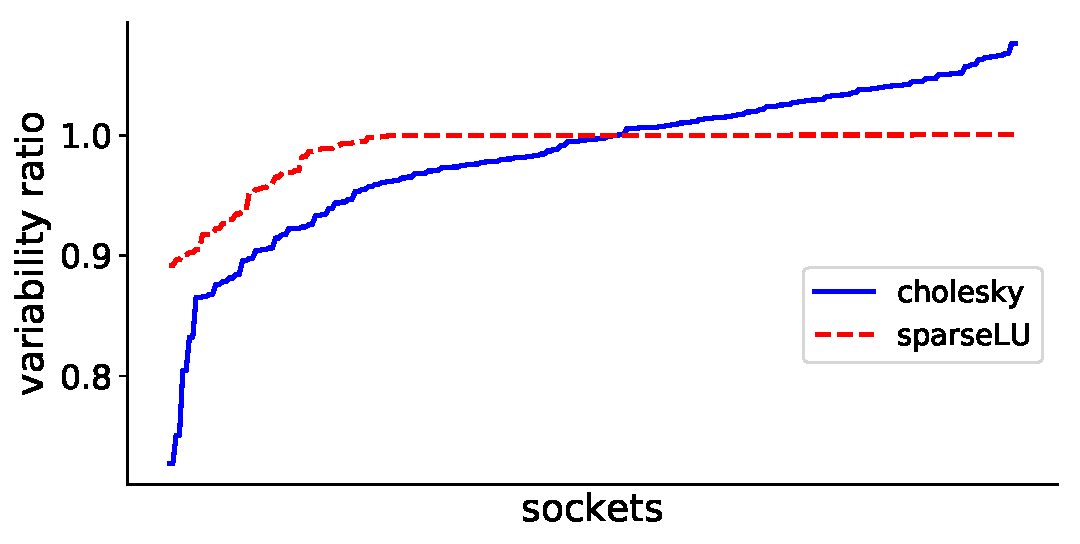
\includegraphics[width=.7\textwidth]{power_aware_job_scheduling/figures/benchmark_var_comparison}
	\caption{Comparison between the variability ratios over all 256 sockets as observed for
\textit{cholesky} and \textit{sparseLU} benchmarks.  Variability ratio here is the
fraction the Power consumption of the benchmark on a given socket, divided by the power
consumption of the same benchmark on a reference socket.  The cpu bound \textit{cholesky} detects variability more precisely than \textit{sparseLU}.}
	\label{fig:bench_var_comparison}
	\vspace{.5cm}
\end{figure}


The PR model's precision is subject to the benchmark application used for measuring the
sockets' manufacturing variability.  Figure \ref{fig:bench_var_comparison} shows the
manufacturing variability for two distinct benchmarks, \textit{cholesky} and
\textit{sparseLU}, as measured by running them on all sockets.  As observer, the two
benchmarks produce different variability ratios.  In the case of \textit{sparseLU}, which
solves the LU factorization problem on a sparse matrix, the observed variability ratio is
on many occasions 1.  This means that this benchmark fails to measure manufacturing
variability effectively and would be able to adjust the original prediction to fit a
socket's variability.  On the other hand, \textit{cholesky}, which is a computation bound
application and stresses the processor more than \textit{sparseLU}, produces a more
precise view of the system's heterogeneity due to manufacturing variability.


\subsection{Variability-Trained Prediction Model}
\label{sec:pmcs_model}

\begin{figure*}[ht!]
	\centering
	\begin{subfigure}[b]{.6\textwidth}
  	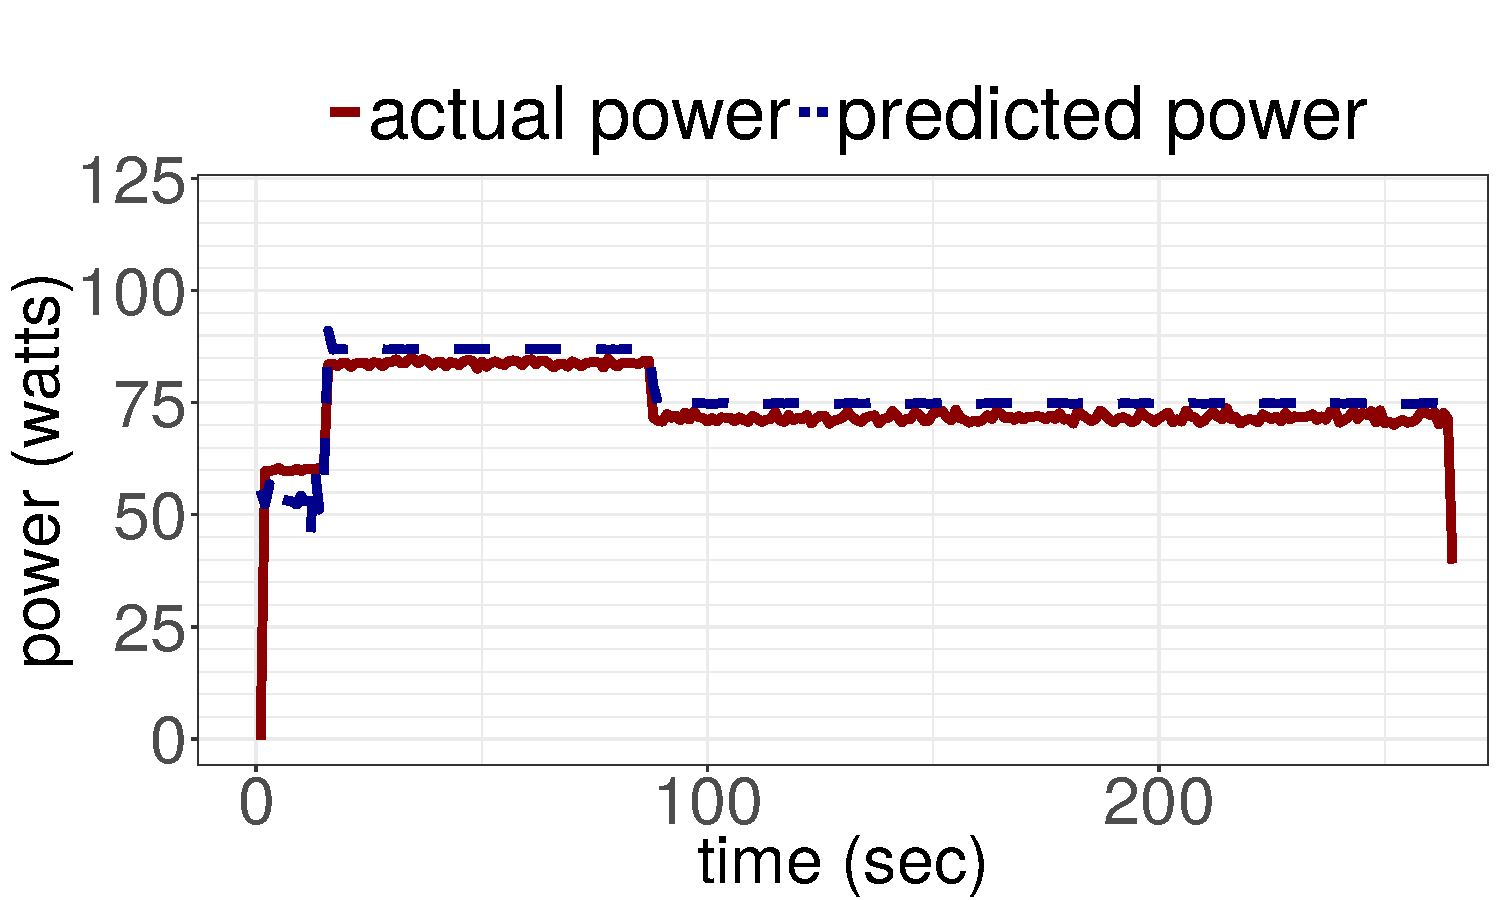
\includegraphics[width=\textwidth]{power_aware_job_scheduling/figures/predict_blackscholes_catalyst45}
  \end{subfigure}%

	\begin{subfigure}[b]{.6\textwidth}
  	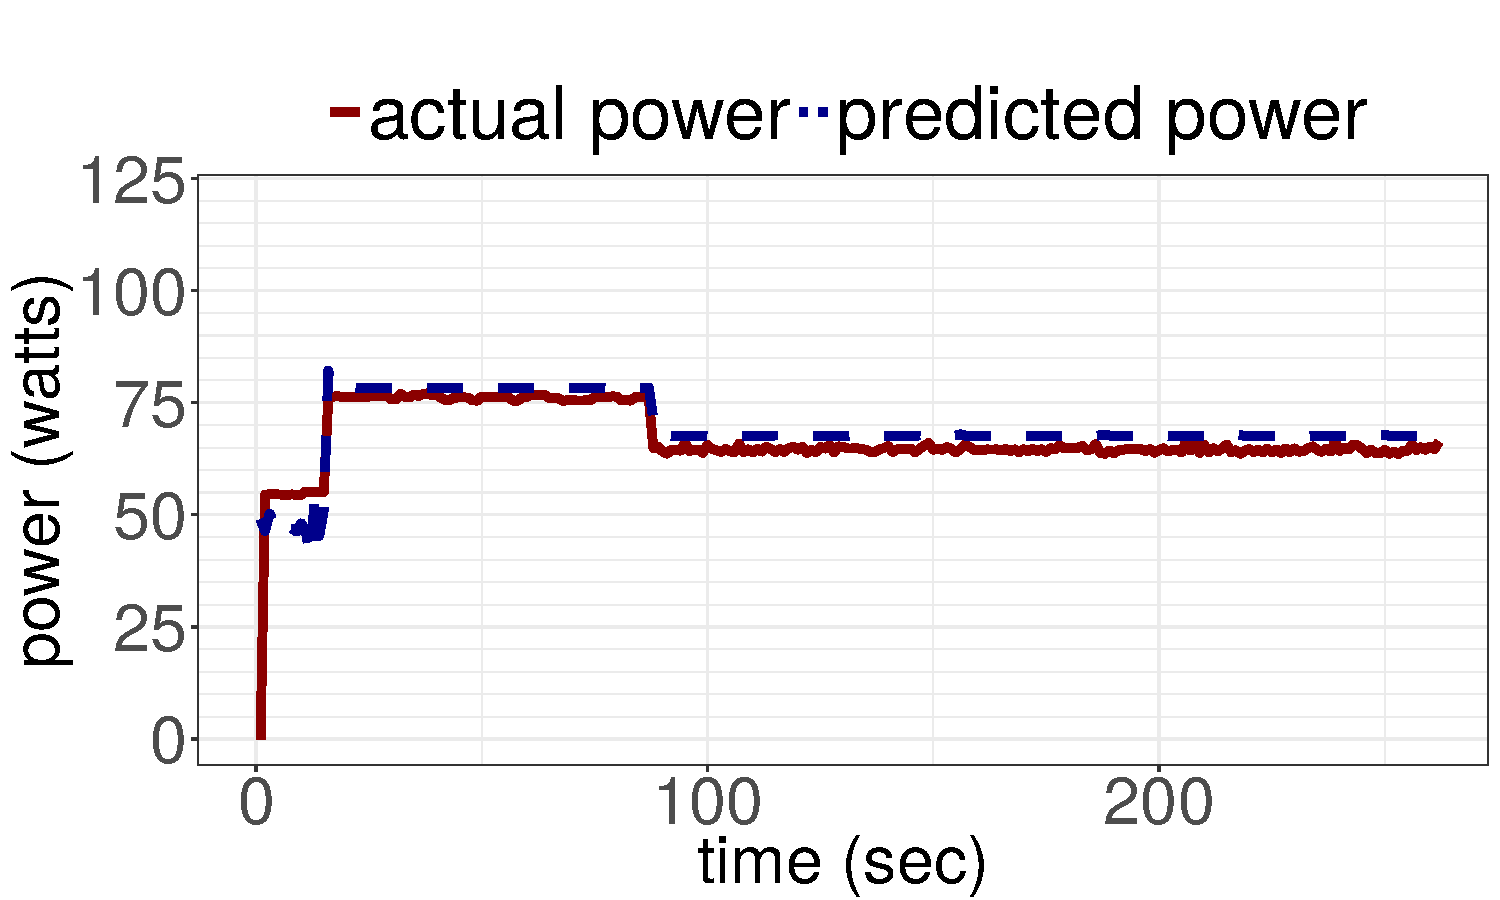
\includegraphics[width=\textwidth]{power_aware_job_scheduling/figures/predict_blackscholes_catalyst79}
	\end{subfigure}%

	\begin{subfigure}[b]{.6\textwidth}
	  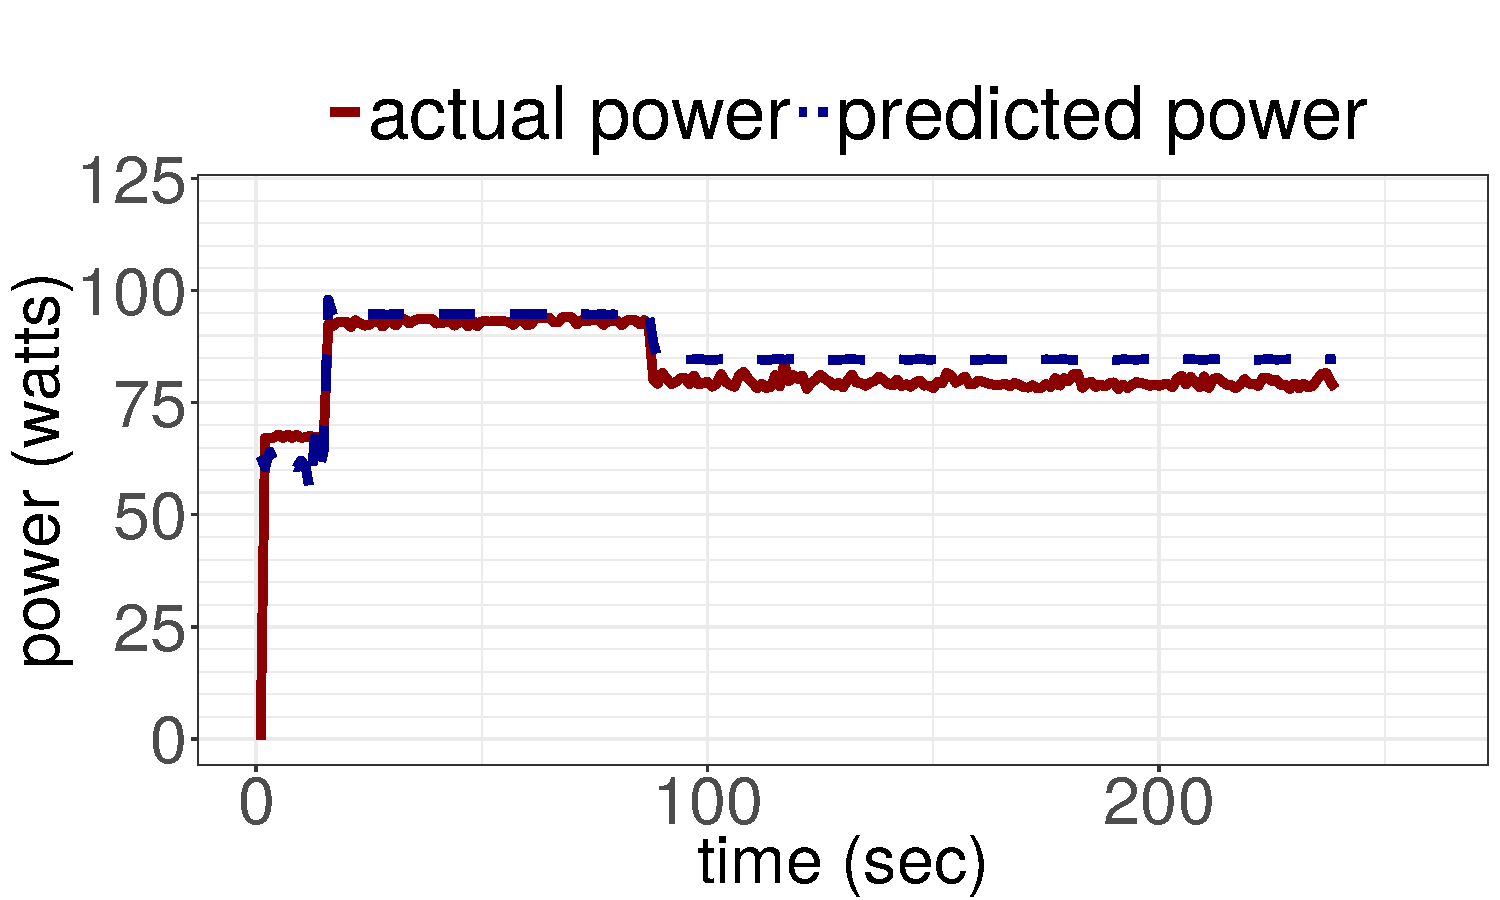
\includegraphics[width=\textwidth]{power_aware_job_scheduling/figures/predict_blackscholes_catalyst239}
	\end{subfigure}%

	\caption{Actual and predicted power consumption, using the PMC-based (Optimized PMC)
model, for \textit{blackscholes} under three distinct sockets. Same CPU chip model is
mounted on all three sockets, utilizing all 12 available cores.}
	\label{fig:prediction_eval}
%	\vspace{-.5cm}
\end{figure*}

\par
Our second model does not assume the impact of manufacturing variability to be independent of the parallel code. 
Instead, it aims at capturing the impact of manufacturing variability on each specific application.
%execution of a particular application on power-capped sockets.  
Due to manufacturing
variability, power consumption differs between sockets, which means that  $W_c$ and
$W_{cores}$ are socket-specific and obtained by solving Equation~\ref{eq:model_formula}
individually for each socket.  In terms of the activity ratio values per application, we
assume them to be invariant across all sockets featuring the same architectural design.
Consequently, the socket-specific Formula~\ref{eq:model_formula} can be extended to
integrate all sockets featuring the same architectural design: 
\begin{equation}
	\label{eq:model_variability_formula}
	P_{socket_i}^{app} = AC^{app} * W_{cores}^{socket_i} + \sum_{c=1}^{N_{comp}} ( AR_c^{app} * W_c^{socket_i} )
\end{equation}
From this formula we can obtain a power prediction of an application running on any chosen
socket, which is characterized in terms of its weights.  For each parallel code we just
need a single run on a generic socket to compute $AR_c$ and $AC$, which are
socket-independent as they are determined by the architectural design.
\par
Figure~\ref{fig:prediction_eval} shows power profiles of the \textit{blackscholes} code
(solid line) running on three different sockets, together with the corresponding predicted
power consumption (dashed line).  Details on the machine and execution setup can be found
in Section~\ref{sec:experimental_setup}.  Figure~\ref{fig:prediction_eval} displays how
the power consumption varies up to 19\% for the same application (from 76W to 96W peak
power), depending on the socket it runs on.  The predicted values capture the power
consumption variability for all cases. 

\subsection{Model Optimization}
To improve the model's precision,  per each application, we consider using only a subset
of architectural components that provides the most accurate results.  This way we
mediate any biasing the training set may have.  All possible combinations of architectural
components are considered and a prediction error is computed for each one.  We use the
Mean Absolute Percentage Error (MAPE) formula for computing this prediction error
\begin{equation}
	\label{eq:mape}
	M = \frac{100}{n}\sum^{n}_{t=1}|\frac{A_t - F_t}{A_t}|
\end{equation}
where $A_t$ and $F_t$ are the actual and predicted values for observation $t$, and $n$ is
the total number of observations.  The model with the lowest error value is chosen for all
future predictions.  This tuning process can be done offline per each targeted application
using data obtained from a single parallel execution.  The same optimization is also
applied to the PR model. From this point on, any mention to the PR and VT models,
references the optimized versions of the models.  The models without the 
optimization mentioned in this paragraph, will be referred to as unoptimized PR and VT
models. Section~\ref{sec:model_validation} shows a detailed evaluation
and validation of both models.

\subsection{Predicting Power for Multi-Node Applications}
For multi-node applications, individual predictions need to be made for each 
MPI process. 
A corresponding model needs to be applied to each socket and process, which has
been trained for each socket individually, producing a different set of weights.  
The result is a prediction of the power consumption of each process and each socket.
For example, if we have an application with N processes and a system with M
sockets, then we make $N \times M$ predictions.

